\chapter{Aufbau \programname}

\section{Architekturbeschreibung}
Im Groben gehalten funktioniert der Daten- und Befehlsfluss im Trufflehog-Entwurf
wie im klassischen \gls{mvc}. Der Presenter aktiviert Services, welche das Model basierend
auf empfangenem Netzwerkverkehr verändert und das View aktualisiert sich am Model.
Da viele Threads im Programm parallel durchlaufen aber dennoch kommunizieren müssen,
verlassen wir uns an einigen Stellen auf das \gls{observerpattern} mit einer
Multi-Thread kompatiblen Datenstruktur.\newline
\newline

\section{Paketbeschreibung}

\subsection{command}
\label{subsec:command}
Das command-Package beinhaltet alle Commands, deren Struktur und die Datenstruktur
\textit{CommandQueue}. Ein Command ist ein Befehl, der auf
dem Model ausgeführt wird. Das heißt alle Objekte, die das Model irgendwie verändern,
werden als Command gekapselt, sodass die Veränderung auf dem Model
ausgeführt werden kann. Es werden alle empfangene Netzwerkpakete
und Benutzerbefehle als Command gekapselt, da diese direkt das Model beeinflussen
indem sie beim Executor ausgeführt werden.
\newline
\newline
Dieses Design hat zwei große Vorteile. Zum einen herscht eine lose Kopplung zwischen
allen Programmteilen, welche das Model verändern wollen und dem Model selbst, was zur Modularität des ganzen
Programms beiträgt. Zum anderen kann man die Commands speichern und zu einem
späteren Zeitpunkt auf einen Snapshot des Modells wieder ausführen um das originale
Model wieder herzustellen. Mehr dazu im
\hyperref[subsubsec:replaylogging]{replaylogging}-Package. Weiter bietet dieses
Design den großen Vorteil das es hohes Erweiterbarkeitspotential hat. Zum Beispiel
könnte man relativ einfach eine undo- und redo-Funktion in einen Command einbauen um
zwischen verschiedene Modelzuständen hin und zurück zu springen. So eine
Funktionalität ist zwar nicht eingeplannt, aber sie währe nicht schwer zu implementieren
an Hand der Command Struktur.
\newline
\newline
Ein potenzielles Problem das auftreten kann, währe wenn ein Command zu lange braucht um
ausgeführt zu werden und so das ganze Programm zum stillstand kommt.
In dem jetztigen Entwurf wird dieses Problem nicht auftreten, da jedes Command
nur schnelle Befehle ausführt wie addEdge() oder ähnliche, welche das System nicht
aufhängen. Jedoch wenn \programname mal so erweitert wird das es doch Commands gibt
die eine lange Ausführungszeit haben, so sollten diese in seperaten Threads
ausgeführt werden um zu verhindern das sich das ganze Programm an einem Command
aufhängt.

\begin{figure}[H]
  \centering
  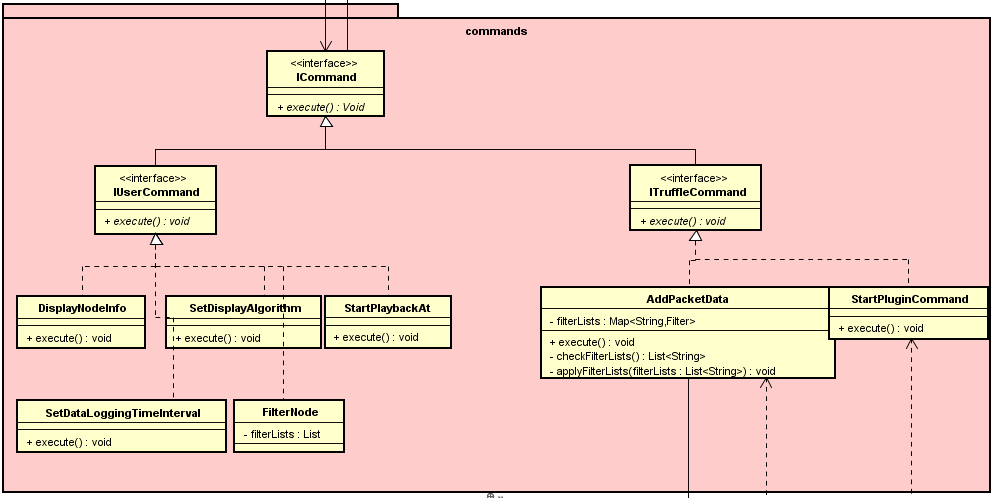
\includegraphics[width=\textwidth]{../diagramimages/commands.png}
  \caption{command-Package}
\end{figure}

Es gibt 2 Arten von Commands, TruffleCommands für die Bearbeitung empfangener
Paketdaten, und UserCommands für die Verwaltung der Benutzeroberflächenbefehle.

      \subsubsection{trufflecommand}
      \label{subsubsec:trufflecommand}
      ***TruffleCommands package image goes here***
      \newline
      \newline
      Jegliche empfangenen Truffles vom \gls{praeprozessor} werden zuerst in Java-Objekt-Truffles umgewandelt, wie
      im \hyperref[subsubsec:truffleprocessor]{truffleprocessor}-Package erklärt. Dort
      werden die erzeugten Java-Truffles in ein Command gesteckt und per \gls{observerpattern}
      wie im \hyperref[subsec:util]{util}-Package beschrieben an alle Interessenten, also die \gls{listener} verschickt.
      \newline
      \newline
      Es gibt nur einen Command-Typen für die empfangen Truffle-\glspl{paket}, nämlich den
      AddPacketDataCommand. Diese Entscheidung wurde getroffen um das Programm einfach
      zu halten. Commands wie AddNode oder AddEdge sind überflüßig, da diese leicht aus
      dem Inhalt des Truffles gelesen werden können.
      \newline
      \newline
      Der PluginNotRunningCommand wird genau dann vom truffleprocessor verschickt, wenn sich \gls{programname}
      nicht mit \gls{sppname} oder einem äquivalenten Plugin verbinden konnte. Wir
      haben die Funktionalität, dass \gls{programname} automatisch \gls{sppname} startet,
      aufgegeben um die beiden Programme unabhängiger zu gestallten und um dem Benutzter
      mehr Freiheit, beispielsweise bei der \gls{praeprozessor}enwahl, zu geben.

      \subsubsection{usercommand}
      \label{subsubsec:usercommand}
      ***UserCommands package image goes here***
      \newline
      \newline

      Wenn der Benutzter eine GUI-Aktion startet, die das Model beeinflusst,
      wird ein entsprechender Command an alle \gls{listener} durch das \gls{observerpattern}, wie im
      \hyperref[subsec:util]{util}-Package beschrieben, verschickt. Für jede mögliche
      GUI-Aktion, welche das Model beeinflusst, gibt es einen passenden Command.
      Diese werden in den ViewControllern aus dem \hyperref[subsec:view]{view}-Package
      an den Executor verschickt.
      //////hier fehlt wer die usercommmands erstellt und losschickt////// **Besser? (von Julian)**

      \subsubsection{queue}
      \label{subsubsec:queue}
      Die Commands, welche beispielsweise der Executor abarbeiten soll, werden in
      einer passenden Datenstruktur zwischengespeichert. Es sind ggf. mehrere
      tatsächliche Queues vorhanden, was nach einem Manager verlangt um nach dem
      Round-Robin-Prinzip faire Verteilung zu ermöglichen. Diese CommandQueue
      ist das empfangende Ende des \gls{observerpattern} an mehreren Stellen unseres
      Programms. Bei Aktualisierung durch einen \gls{notifier} geht dieser alle
      seine \gls{listener} durch und fügt bei jedem in genau eben diese
      CommandQueue das neue Command-Objekt ein. Die Implementierung der Queues
      als BlockingQueue ermöglicht in diesem Fall die Kommunikation zwischen Threads.

\subsection{service}
\label{subsec:service}

Im service-Package befinden sich alle durchlaufenden Threads von \gls{programname},
mit Ausnahme vom \hyperref[subsec:view]{view}, das ein eigenes Package zur verzögerungsfreien Darstellung ist, und dem
main-Thread. Jedes Unterpackage kapselt dabei genau eine selbständig laufende Funktionalität, meist eine pro Thread. Unten ist erklärt, was genau jedes Unterpackage macht.

\begin{figure}[H]
  \centering
  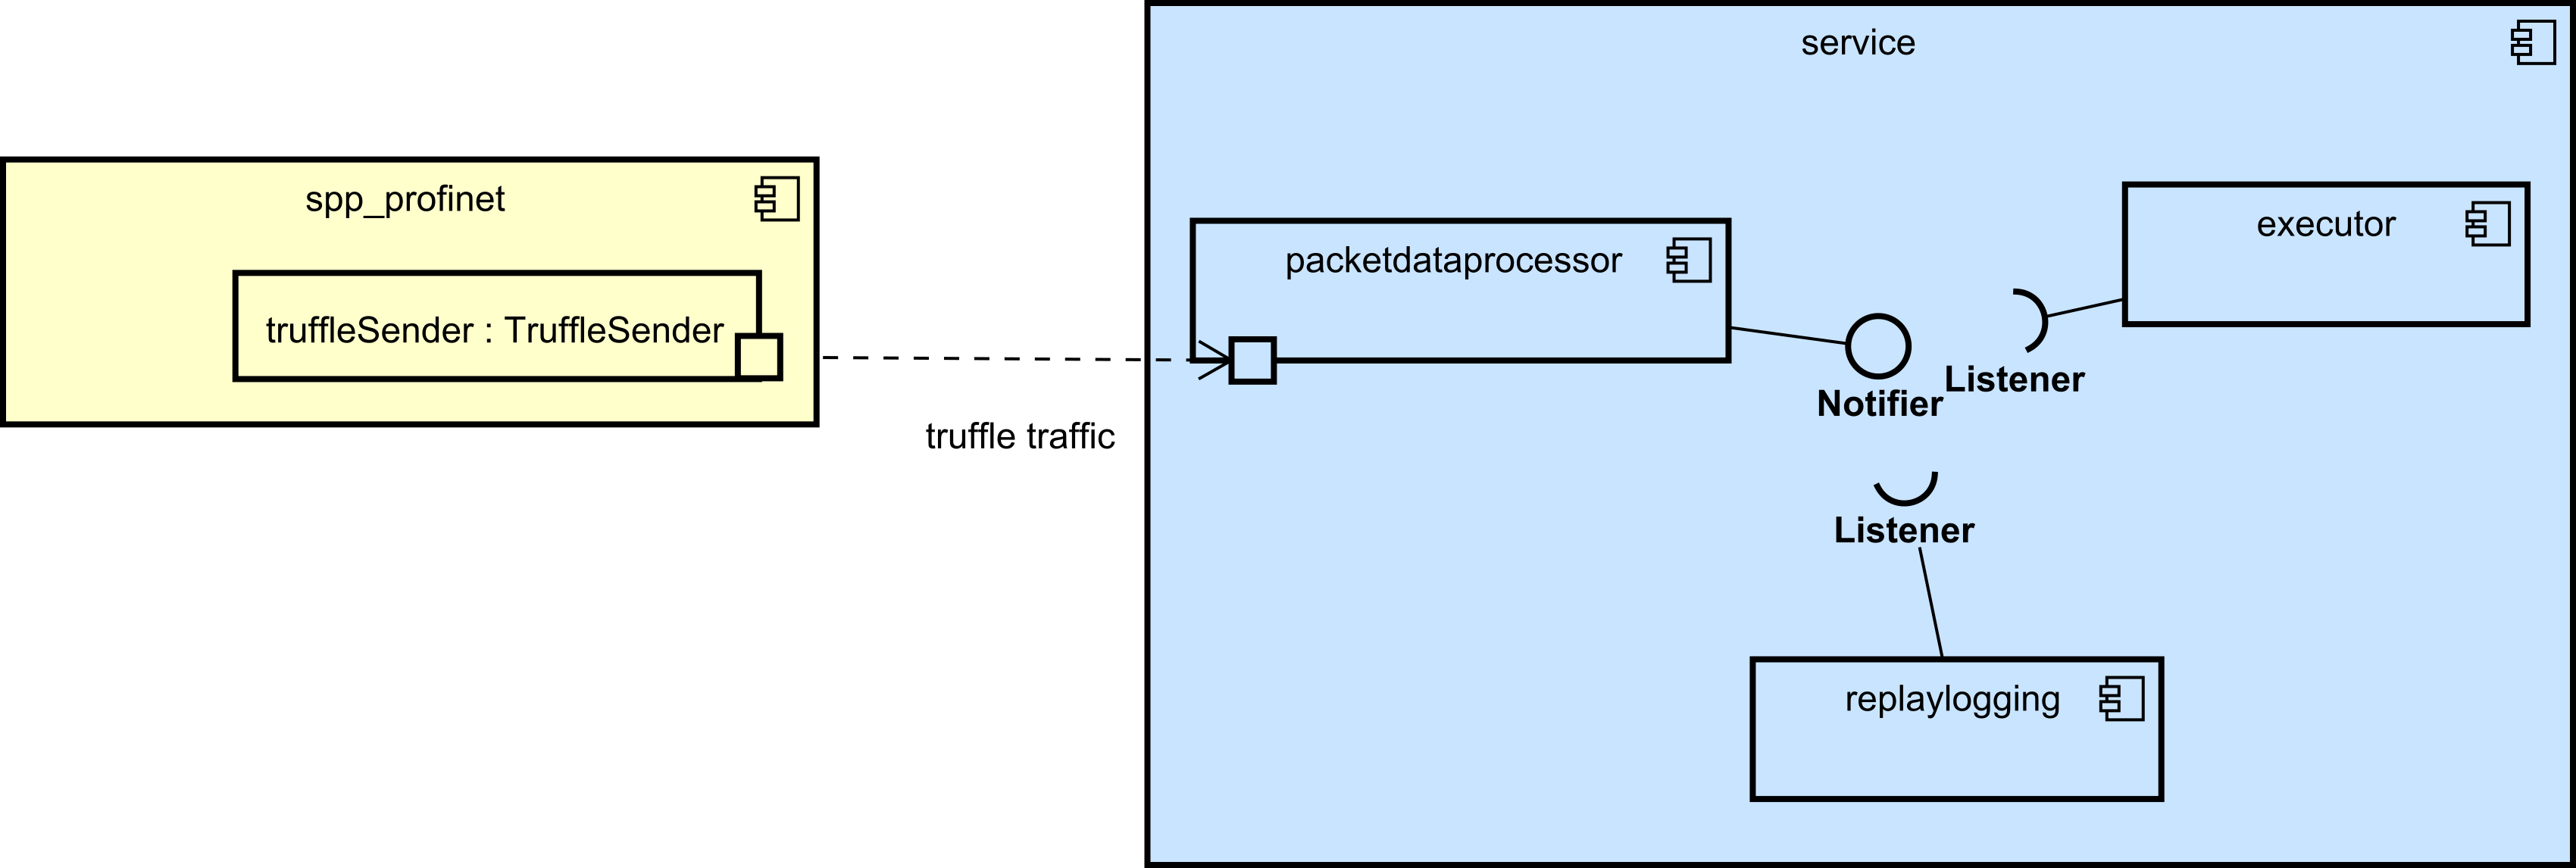
\includegraphics[width=\textwidth]{../diagramimages/service.png}
  \caption{service-Package}
  \medskip
\end{figure}

    \subsubsection{truffleprocessor}
    \label{subsubsec:truffleprocessor}

    *** truffleprocessor image here ***
    \newline
    \newline
    Der truffleprocessor-Service läuft konstant im Hintergrund, in einem eigenen Thread,
    und empfängt die im \gls{sppname} erstellten Truffles.
    Diese packt er in ein Java-Truffle-Objekt, welches dann wiederum von dem
    \textit{TruffleReciever} in ein Command gesteckt wird. Da der \textit{TruffleReciever}
    auch ein \gls{notifier} ist, verschickt er den Command auch gleich an
    alle registrierten \gls{listener}, sodass der CommandExecutor die bekommt wo die Commands
    als nächstes auf dem Model angewandt werden.

    \subsubsection{replaylogging}
    \label{subsubsec:replaylogging}

    *** replaylogging image here ***
    \newline
    \newline

    Der replaylogging-Service besteht aus 2 Prozessen die jeweils ihre eigenen Threads haben//same//.
    Der erste ist der \textit{ReplayLogSaveService} und kümmert sich um das speichern das aktuellen
    Graphen. Der zweite ist der \textit{ReplayLogLoadService} und kümmert sich um das
    wiederherstellen eines gespeicherten Graphen.
    \newline
    \newline
    Der \textit{ReplayLogSaveService} läuft konstant im Hintergrund und empfängt alle
    vom \textit{TruffleReciever} verschickten Commands. Diese werden alle X
    Sekunden (vom Benutzter festlegbar) komprimiert und in eine Liste gepackt.
    Komprimiert heißt, dass viele Commands, die das selbe tun, in ein Command
    gepackt werden. Zusätzlich zu den Commands wird auch noch ein Snapshot
    von dem aktuellen Graphen gemacht, der dann zusammen mit der erstellten
    Command-Liste in ein ReplayLog-Objekt getan wird. Dieses
    ReplayLog-Objekt wird dann von Java serialisiert und gespeichert.
    \newline
    \newline
    Diese Logs können zu einem späteren Zeitpunkt wieder geladen werden um den
    Graphen wiederherzustellen. Dazu ist der \textit{ReplayLogLoadService} da. Wenn
    der User die Replayfunktion aktiviert, fängt der ReplayLogLoadService an die
    ReplayLogs zu laden. Dann wird in der view der Snapshotgraph angezeigt
    und die gespeicherten Commands aus dem ReplayLog werden auf
    diesem Snapshot angewandt. Der ReplayLogLoadService kontrolliert somit die
    Wiedergabe des alten Graphen und kann sogar hin und her zwischen Snapshots
    springen (momentan nicht zwischen einzelnen Commands, da dieses keine undo-
    und redo-Funktion besitzten).
    \newline
    \newline
    Der ReplayLogLoadService läuft in seinem eigenen Thread, weil er sich darum
    kümmert das immer genügend Daten im Speicher liegen. In anderen Worten, er
    buffert die Replaylogs vor damit sich der Graph bei dem Benutzter flüssig
    abspielt.

    \subsubsection{executor}
    \label{subsubsec:executor}

    *** executor image here ***
    \newline
    \newline

    Der executor-Service läuft auch wieder konstant im Hintegrund in seinem
    eigenen Thread. Er ist ein \gls{listener} der sowohl bei dem TruffleReciever aus dem
    \hyperref[subsubsec:truffleprocessor]{truffleprocessor}-Package als
    auch bei den view-Controllern aus dem \hyperref[subsec:view]{view}-Package
    registriert ist. D.h. er bekommt, wie das \hyperref[subsubsec:replaylogging]{replaylogging},
    alle \hyperref[subsubsec:trufflecommand]{TruffleCommands} und führt diese
    dann auf dem aktuellen Model aus.
    \newline
    \newline
    In \gls{programname} gibt es zwei Instanzen vom Executor. Die erste bearbeitet
    den aktuellen Graphen, und die zweite bearbeitet die Snapshot-Instanz, falls
    eine existiert. So kann der aktuelle Graph auf dem neusten Stand bleiben, während
    gleichzeitig der Benutzter einen alten Graphen aus
    ReplayLogs rekonstruiert anschaut.


\subsection{presenter}
\label{subsec:presenter}

Der presenter ist für den Aufbau von \gls{programname}, also das
Initialisieren, Instanziieren und Referenzieren aller Programmelemente zuständig.
Er ist sozusagen der \"glue code\" von \gls{programname}.

\begin{figure}[H]
  \centering
  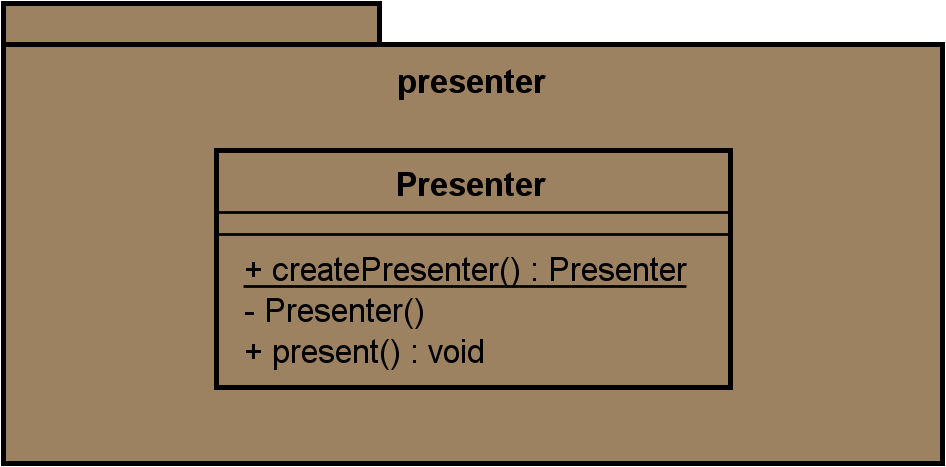
\includegraphics[width=\textwidth]{../diagramimages/presenter.png}
  \caption{presenter-Package}
\end{figure}

Er wird im main-Thread von der main-Klasse erzeugt und ruft alle Konstruktoren auf.
In anderen Worten baut er \gls{programname} auf.

\subsection{util}
\label{subsec:util}

Im util-Package befinden sich Klassen die komplet von \gls{programname} abgekoppelt
sind. D.h. sie werden nur als Ressource, wie eine Liste, verwändet und nehmen kein
Bezug auf das Programm.

\begin{figure}[H]
  \centering
  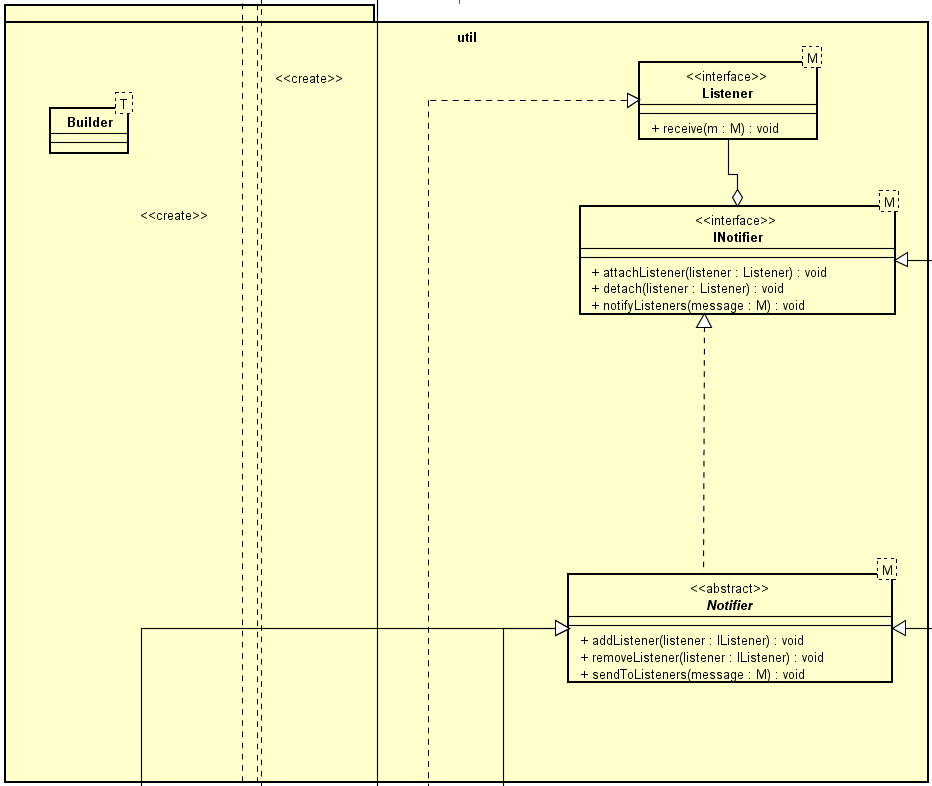
\includegraphics[width=\textwidth]{../diagramimages/util.png}
  \caption{util-Package}
\end{figure}

Konkret befinden sich 3 Klassen im util-Package, die alle zusammen eine
Variation des Observer Patterns realisieren. Der \textit{Notifier} ist dazu da
ein beliebiges Objekt zu verschicken, deshalb der Generic. Er ist das subjekt aus
dem Observerpattern.
\newline
\newline
Der \textit{INotifier} existiert für den Fall, dass ein
Objekt ein Notifier sein muss, aber nicht Notifier vererben kann, weil es
schon eine andere Klasse vererbt. Dieses Problem tritt beispielsweise in der
\hyperref[subsec:view]{view} auf, wo viele Klassen GUI aktionen als Commands
gekapselt an den Executor schicken und gleichzeitig JavaFX Klassen vererben müssen.
Um dieses Problem zu lösen implementieren diese Klassen das INotifer interface
und haben ein Hilfsobjekt das Notifier vererbt und sommit die gewünschte Funktionalität
bietet.
\newline
\newline
Der \textit{Listener} ist der Observer aus dem Obsever Pattern. Hier ist nichts
besonderes, mit Ausnahme der receive Methode bei der wir einen Parameter eingeführt
haben dammit der Listener das versendete Objekt des Notifiers auch empfangen kann.
Zu diesem Zweck existiert auch wieder ein Generic.
\newline
\newline
Dieses Observer Pattern verwaltet das verschicken und empfangen von Commands in
\gls{programname}. In anderen worten, jede Klasse die Commands verschickt ist ein
INotifier, und jede Klasse die Commands empfängt ist ein Listener. Dieses Design
hat große Vorteile, da die Sender und die Empfänger komplet voneinander abgekoppelt
sind. Der \hyperref[subsec:presenter]{Presenter} registriert die Listeners am
Anfang bei den Notifiern, somit kennt der Listener nicht seinen Notifier, und der
Notifier weiss nicht, was sich hinter einem Listener versteckt. Durch dieser losen
Kopplung ist es einfach \gls{programname} um einen zusätzlichen Service zu erweitern
da kein Service wirklich von einem anderen abhängt.
\newline
\newline
Ein Beispiel dieser losen Kopplung kann man zwischen dem
\hyperref[subsubsec:truffleprocessor]{truffleprocessor}-Package, dem
\hyperref[subsubsec:executor]{executor}-Package, und dem
\hyperref[subsubsec:replaylogging]{replaylogging}-Package finden. Hier erstellt
der Truffleprocessor neue Commands die sowohl von dem Executor als auch von dem
ReplayLogSaveService empfangen werden sollen. Obwohl die 3 Packages sehr viel
mit einander zu tun haben, kenne sie sich gegenseitig nicht. Dieses Design
führt zur modularität von \gls{programname} hinzu.

\subsection{model}
\label{subsec:model}

Das Model beinhaltet jegliche Datenstrukturen die von \gls{programname} genutzt
werden. Zum beispiel ist der Graph der im View angezeigt wird hier enthalten, sowohl
als auch alle Konfigurationen die der Benutzer eingestellt hat. Wir haben die
Designentscheidung getroffen, dass das Model keine ausführungs Logik enthält.
D.h. es besitzt kein eigenen Thread und wird wie eine Art Ressource von den
\hyperref[subsec:service]{Services} und dem \hyperref[subsec:view]{View} verwändet.

\begin{figure}[H]
  \centering
  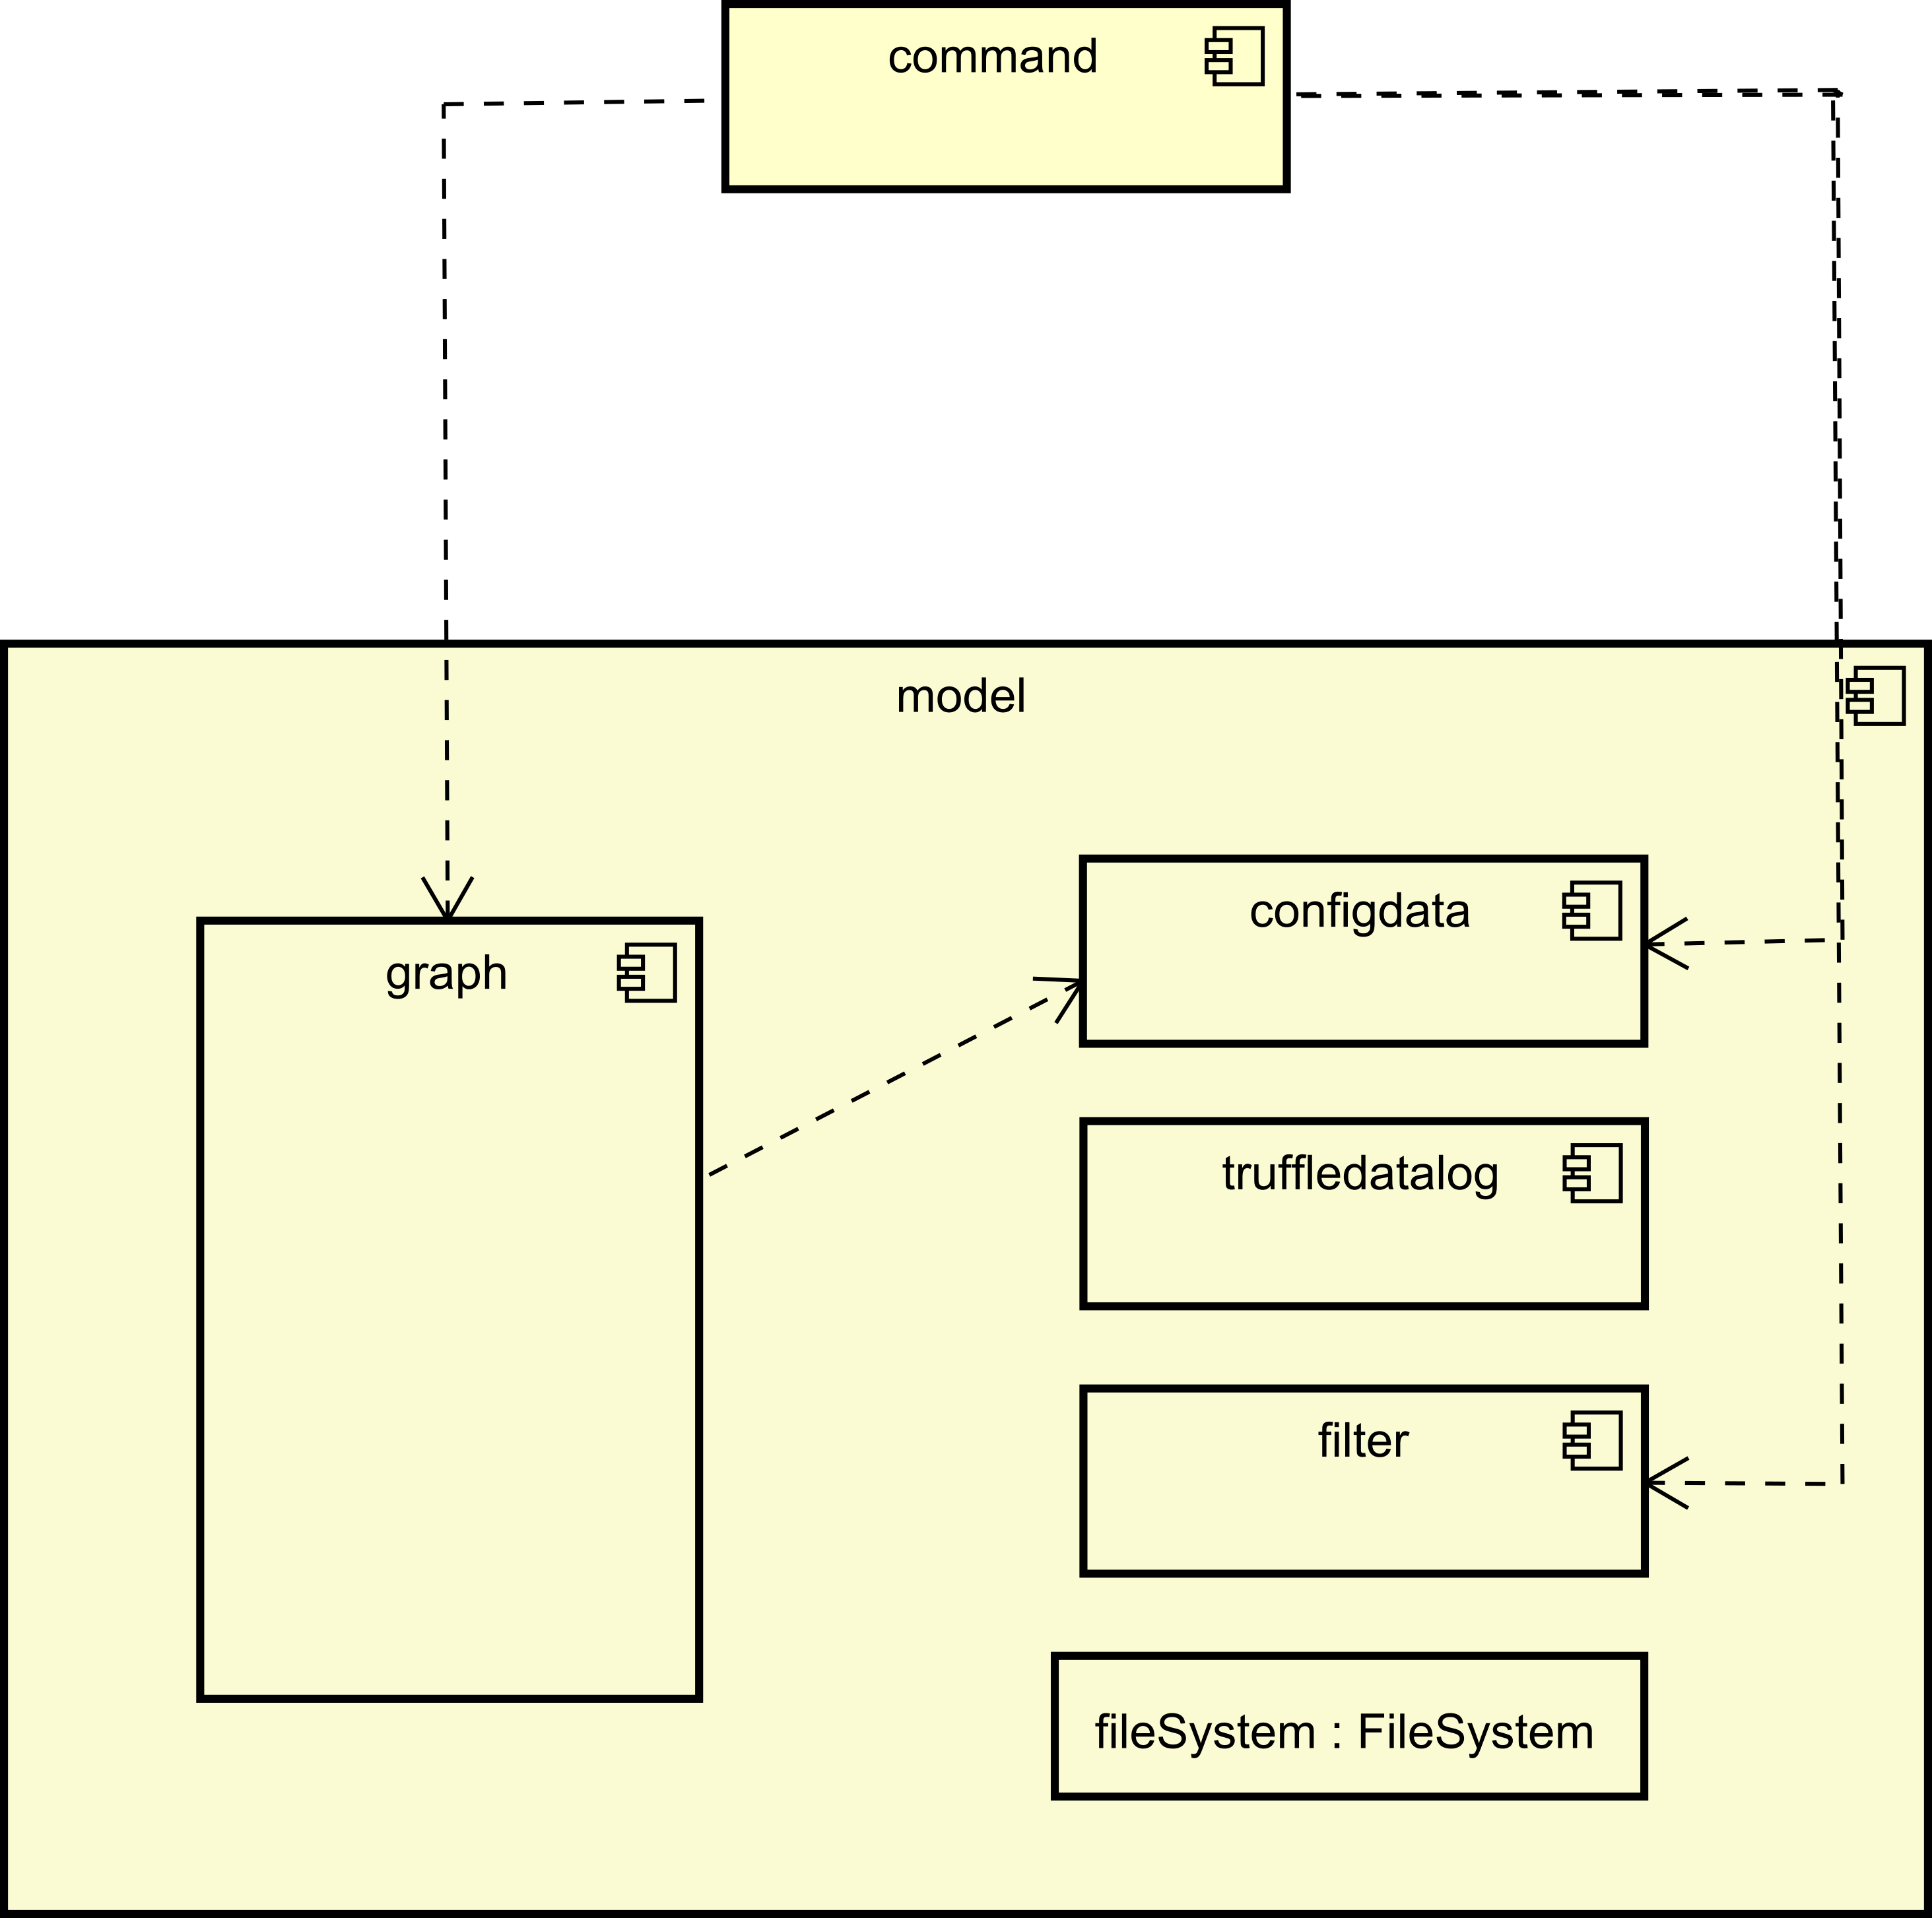
\includegraphics[width=\textwidth]{../diagramimages/model.png}
  \caption{model-Package}
\end{figure}

    \subsubsection{graph}
    \label{subsubsec:graph}
    ***graph package image goes here (maybe? if its not too big)***
    \newline
    \newline
    Dieses Unterpackage macht das eigentliche Modell aus. Der gesamte Graph sowie
    all seine möglichen Layouts, entsprechende Interfaces und ein Proxy aus dem
    \gls{proxypattern} für die Entkopplung sind hier enthalten.

    \subsubsection{filter}
    \label{subsubsec:filter}
    ***filter package image goes here***
    \newline
    \newline
    Das filter-Package beinhaltet eine \textit{Filter} Klasse die in der Lage ist,
    Knoten basierend auf Benutztergegebenenkriterien zu klassifizieren. Verschiedene
    Klassifikationen werden verschieden in der View dargestellt. So kann
    Beispielsweise eine Blacklist oder Whitelist erstellt werden.
    Natürlich kann der Benutzer basierend auf \gls{ip}- und \gls{mac}-Addressräumen,
    Gerätenamen oder Knotenselektionen seine eigenen Filter erstellen.

    \subsubsection{configdata}
    \label{subsubsec:configdata}
    ***configdata package image goes here***


    \subsubsection{graphlog}
    \label{subsubsec:graphlog}
    ***graphlog package image goes here***


\subsection{view}
\label{subsec:view}

\subsection{interactors}
\label{subsec:interactors}
